% glyph-metrics.tex
%
% written 2022 by Werner Lemberg <wl@gnu.org>


% This file contains graphics used for the 'FreeType Glyph Conventions'
% tutorial, part 3, 'Glyph Metrics'.


% Here is one possibility to convert this LaTeX file to both PNG and SVG
% formats.
%
%   xelatex glyph-metrics.tex
%
%   pdftoppm -png -f 1 -l 4 -r 120 glyph-metrics.pdf glyph-metrics
%   optipng glyph-metrics-*.png
%
%   for i in 1 2 3 4; do
%     pdf2svg glyph-metrics.pdf glyph-metrics-$i.svg $i
%   done


\documentclass[tikz, border=3mm]{standalone}

\usepackage{libertinus}

\usetikzlibrary{
  calc,
  decorations,
  positioning
}


% Node styles.
\tikzset{
  % For dimensionless point nodes.
  dummy/.style={
    inner sep=0pt,
    outer sep=0pt},
%
  % For thick curves with one arrow.
  axis/.style={
    line width=4pt,
    -latex},
%
  % For fat dots.
  dot/.style={
    minimum size=14pt,
    circle,
    fill},
%
  % 'Elastic dashes' adapt spaces between dashes to the line length so that
  % the last dash doesn't get cut off partially.
  %
  % Taken from
  % https://tex.stackexchange.com/questions/133271/can-tikz-dashed-lines-emulate-pstricks-dashed-lines
  elastic dash/.code args={on #1 off #2}{
    % Use csname so catcode of @ doesn't have do be changed.
    \csname tikz@addoption\endcsname{%
      \pgfgetpath\currentpath
      \pgfprocessround{\currentpath}{\currentpath}%
      \csname pgf@decorate@parsesoftpath\endcsname
        {\currentpath}{\currentpath}%
      \pgfmathparse{\csname pgf@decorate@totalpathlength\endcsname-#1}%
      \let\rest=\pgfmathresult
      \pgfmathparse{#1+#2}%
      \let\onoff=\pgfmathresult
      \pgfmathparse{max(floor(\rest/\onoff), 1)}%
      \let\nfullonoff=\pgfmathresult
      \pgfmathparse{max((\rest-\onoff*\nfullonoff)/\nfullonoff+#2, #2)}%
      \let\offexpand=\pgfmathresult
      \pgfsetdash{{#1}{\offexpand}}{0pt}}},
%
  % For main curves.
  line/.style={
    line width=2pt},
%
  % For auxiliary, dashed curves.
  dashed line/.style={
    elastic dash=on 6pt off 6pt,
    line},
%
  % For displaying node coordinates.
  coordinate/.style={
    font=\Huge},
%
  % For explanations.
  description/.style={
    font=\Huge\itshape},
%
  % For curves with one arrow.
  direction/.style={
    line,
    -latex},
  % For curves with two arrows.
  span/.style={
    line,
    latex-latex},
%
  % For (invisible) boxes displaying advances.
  box/.style={
    inner sep=0pt,
    font=\fontsize{150pt}{0pt}\selectfont},
%
  % For displaying horizontal advances.
  hbox/.style={
    box,
    outer sep=0pt,
    anchor=base west},
%
  % For displaying vertical advances.
  vbox/.style={
    box,
    outer sep=10pt,
    anchor=north},
%
  % We want to draw a tight bounding box around the ink of glyph 'g', which
  % needs some manual work.  We use `inner xsep` with a negative value to
  % remove the glyph's side bearings.  Since the left and the right side
  % bearings are not equal, we need `\hspace` as an additional compensation.
  % For the top and bottom side bearings, adjusting `inner ysep` is
  % sufficient.
  glyph g/.style={
    draw,
    line,
    inner xsep=-6pt,
    inner ysep=0pt,
    outer sep=0pt,
    font=\fontsize{300pt}{0pt}\selectfont,
    execute at end node={\hspace{-3pt}g}},
%
  % For filled squares
  %
  % Taken from
  % https://tex.stackexchange.com/questions/300098/draw-a-node-as-a-square-with-tikz
  square/.style={
    fill,
    minimum size=9pt,
    inner sep=0pt}
}


\newcommand*{\LastLoopValue}{No value}


%%%%%%%%%%%%%%%%%%%%%%%%%%%%%%%%%%%%%%%%%%%%%%%%%%%%%%%%%%%%%%%%%%%%%%%%%%%%%

\begin{document}

% Horizontal advance widths.

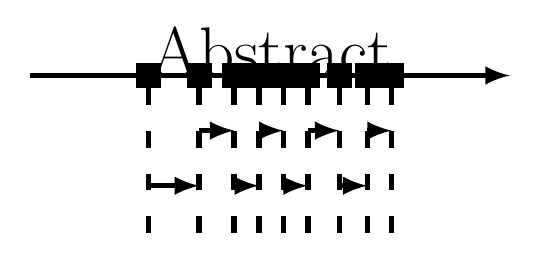
\begin{tikzpicture}
  % Put dummy node 'glyph0' at the left edge.
  \node[dummy] (glyph0) {};
  \node[square] (square0) at (glyph0.base west) {};
  \draw[line] (glyph0.base west) -- +(-1.5,0);
  \draw[dashed line] (square0) -- +(0,-2);

  % Loop over all characters; the nodes have the name 'glyph1', 'glyph2',
  % etc.
  \foreach \g [count=\i, remember=\i as \lasti] in {A, b, s, t, r, a, c, t}
    {\node[hbox] (glyph\i) at (glyph\lasti.base east) {\g};
     \node[square] (square\i) at (glyph\i.base east) {};

     \draw[dashed line] (square\i) -- +(0,-2);
     \draw[direction]
       let
         \p{offset}=(0,{-0.7 * mod(\i, 2) - 0.7})
       in
         ($(glyph\i.base west) + (\p{offset})$)
           -- ($(glyph\i.base east) + (\p{offset})$);

     \draw [line] (glyph\i.base west) -- (glyph\i.base east);

     \xdef\LastLoopValue{\i}
    }

  \draw[direction] (glyph\LastLoopValue.base east) -- +(1.5,0);
\end{tikzpicture}


% Vertical advance widths.

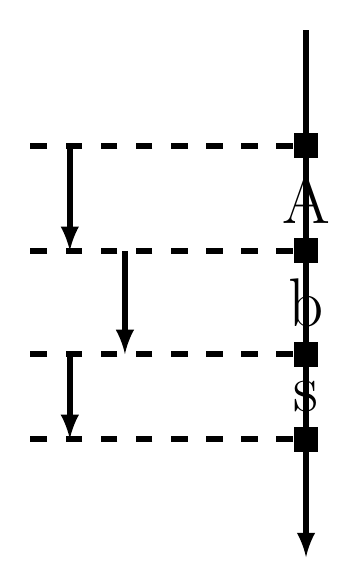
\begin{tikzpicture}
  \node[dummy] (glyph0) {};
  \node[square] (square0) at (glyph0.north) {};
  \draw[line] (glyph0.south) -- +(0,1.5);
  \draw[dashed line] (square0) -- +(-3.5,0);

  \foreach \g [count=\i, remember=\i as \lasti] in {A, b, s}
    {\node[vbox] (glyph\i) at (glyph\lasti.south) {\g};
     \node[square] (square\i) at (glyph\i.south) {};

     \draw[dashed line] (square\i) -- +(-3.5,0);
     \draw[direction]
       let
         \p{offset}=({-0.7 * mod(\i, 2) - 2.3},0)
       in
         ($(glyph\i.north) + (\p{offset})$)
           -- ($(glyph\i.south) + (\p{offset})$);

     \draw [line] (glyph\i.north) -- (glyph\i.south);

     \xdef\LastLoopValue{\i}
    }

  \draw[direction] (glyph\LastLoopValue.south) -- +(0,-1.5);
\end{tikzpicture}


% Horizontal metrics.

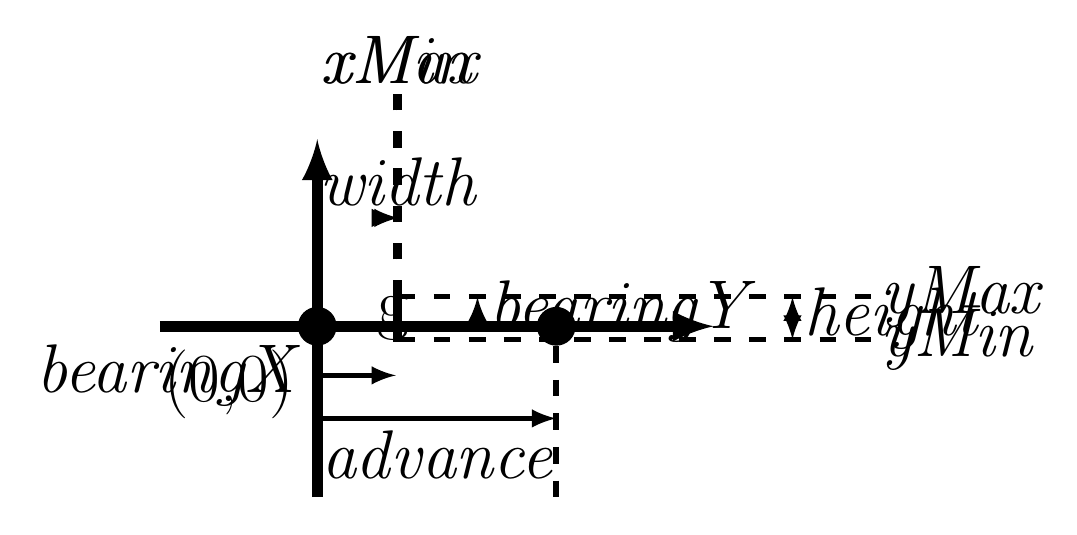
\begin{tikzpicture}
  \node [glyph g,
         anchor=base west] (glyph) at (1,0) {};

  \draw[axis] (-2,0) -- ($(glyph.base east) + (4,0)$);

  \node (bottom edge) at ($(glyph.south west) + (-1,-2)$) {};
  \draw[axis] (bottom edge.center) -- ($(glyph.north west) + (-1,2)$);

  \node[dot, label={[coordinate] below left:(0,0)}] at (0,0) {};
  \node[dot] (advance width) at ($(glyph.base east) + (2,0)$) {};

  \node[description] (xMin) at ($(glyph.north west) + (0,3)$) {xMin};
  \draw[dashed line] (glyph.north west) -- (xMin);

  \node[description] (xMax) at ($(glyph.north east) + (0,3)$) {xMax};
  \draw[dashed line] (glyph.north east) -- (xMax);

  \draw[span] ($(glyph.north west) + (0,1)$)
                -- ($(glyph.north east) + (0,1)$)
              node [midway, above, description] {width};
  \draw[direction] ($(glyph.north west) + (-1,-1)$) -- +(1,0)
                   node [anchor=east, pos=0, description] {bearingX\/};

  \draw[dashed line] (advance width) -- (bottom edge -| advance width);
  \draw[direction] ($(bottom edge) + (0,1)$)
                     -- ($(bottom edge -| advance width) + (0,1)$)
                   node [midway, below, description] {advance};

  \node[description,
        anchor=west] (yMax) at ($(glyph.north east) + (6,0)$) {yMax};
  \draw[dashed line] (glyph.north east) -- (yMax);

  \node[description,
        anchor=west] (yMin) at ($(glyph.south east) + (6,0)$) {yMin};
  \draw[dashed line] (glyph.south east) -- (yMin);

  \draw[direction] ($(glyph.base east) + (1,0)$)
                     -- ($(glyph.north east) + (1,0)$)
                   node [midway, right, description] {bearingY};
  \draw[span] ($(glyph.south east) + (5,0)$)
                -- ($(glyph.north east) + (5,0)$)
              node [midway, right, description] {height};
\end{tikzpicture}


% Vertical metrics.

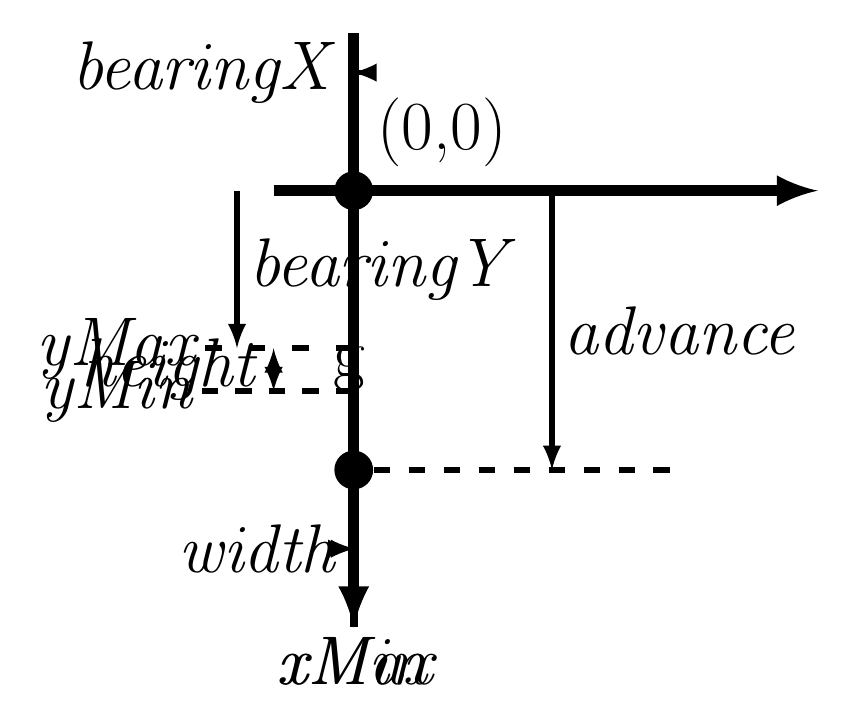
\begin{tikzpicture}
  \node [glyph g,
         anchor=north] (glyph) at (0,-2) {};

  \node (right edge) at ($(glyph.north east) + (6,2)$) {};
  \draw[axis] ($(glyph.north west) + (-1,2)$) -- (right edge);

  \draw[axis] (0,2) -- ($(glyph.south) + (0,-3)$);

  \node[dot, label={[coordinate] above right:(0,0)}] at (0,0) {};
  \node[dot] (advance height) at ($(glyph.south) + (0,-1)$) {};

  \node[description] (yMax) at ($(glyph.north west) + (-3,0)$) {yMax};
  \draw[dashed line] (glyph.north west) -- (yMax);

  \node[description] (yMin) at ($(glyph.south west) + (-3,0)$) {yMin};
  \draw[dashed line] (glyph.south west) -- (yMin);

  \draw[span] ($(glyph.north west) + (-1,0)$)
                -- ($(glyph.south west) + (-1,0)$)
              node [midway, left, description] {height\/};

  \draw[direction] ($(glyph.north east) + (-1.5,2)$) -- +(0,-2)
                   node [midway, right, description] {bearingY};

  \draw[dashed line] (advance height)
                       -- ($(right edge |- advance height) + (-2,0)$);
  \draw[direction] ($(right edge) + (-3.5,0)$)
                     -- ($(right edge |- advance height) + (-3.5,0)$)
                   node [midway, right, description] {advance};

  \node[description,
        anchor=north] (xMin) at ($(glyph.south west) + (0,-3)$) {xMin};
  \draw[dashed line] (glyph.south west) -- (xMin);

  \node[description,
        anchor=north] (xMax) at ($(glyph.south east) + (0,-3)$) {xMax};
  \draw[dashed line] (glyph.south east) -- (xMax);

  \draw[span] ($(glyph.south west) + (0,-2)$)
                -- ($(glyph.south east) + (0,-2)$)
              node [anchor=east, pos=0, description] {width\/};

  \draw[dashed line] (glyph.north west) -- +(0,4);
  \draw[direction] (0,1.5) -- (glyph.north west |- 0,1.5)
                   node [left, description] {bearingX\/};
\end{tikzpicture}

\end{document}
